% CHAPTER 1
\chapter{WIND TURBINE MODELLING}
\label{chp:3}

\section{VARIABLE SPEED PMSG WIND TURBINES}

The share of variable speed PMSG wind turbines is increasing worldwide due to the high efficiency and torque density. This type of wind turbines are equipped with full-scale power electronics which enable the turbine to have wide speed range. Even though the permanent magnet price fluctuates with time, the reliability and high efficiency of this type of turbine increase its share in the market.

 \begin{figure}[h!]
	\centering
	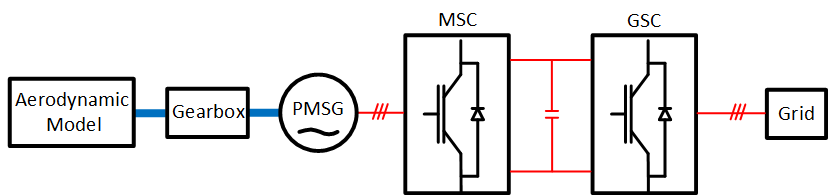
\includegraphics[width=1\linewidth]{Windmodel.png}
	\caption{Variable Speed Geared Wind Turbine Model}
	\label{varspeedpmsg}
\end{figure} 

Figure \ref{varspeedpmsg} shows the modelling of variable speed wind turbine. The aerodynamic sub-model includes turbine structure that captures power from the wind. The gearbox establishes the connection between wind turbine and PMSG. In this type of wind turbines, PMSG is not directly connected to grid so that the turbine speed is independent from the grid frequency. Therefore, back-to-back converter is used between generator and the electrical grid. The converter which is connected to PMSG is called Machine Side Converter (MSC) meanwhile the one connected to grid is called Grid Side Converter(GSC).

\subsection{Aerodynamic Model}
Aerodynamic model is the sub-model that captures power from the wind. The output of this block is the aerodynamic torque that rotates the turbine. However, the wind speed is not the only input. Turbine speed and pitch angle are also the inputs of the system since they affect the mechanical power that is captured from the wind.\par
The aerodynamic power of wind is given in Equation \ref{windpower} where $\rho_{air}$ is air density in $kg/cm^{3}$, $R$ is the blade radius in $m$ abd $v_{WIND}$ is the wind speed in $m/s$. Note that this is the available power of the air that is striking the turbine swept area and it is not possible to extract that amount of energy. Otherwise, the air would be standstill behind the wind turbine \cite{Ackermann2005a}.
\begin{equation}
P_{WIND}=0.5\rho_{air}\pi R^{2} v_{WIND}^{3}
\label{windpower}
\end{equation}
The wind turbine captures a fraction of the available wind power that is denominated as power coefficient $C_{p}$. Therefore, turbine power captured from wind can be found with the Equation \ref{turbinepower}.
\begin{equation}
P_{TUR}=C_{P}P_{WIND}
\label{turbinepower}
\end{equation}

Power coefficient determines the amount of power and it is a non-linear function of the tip speed ratio, $\lambda$ and pitch angle, $\beta$. Tip speed ratio is a parameter proportional with turbine speed. It can be defined as the ratio of the speed in the turbine tip to the wind speed as in the Equation \ref{tipspeed}. Power coefficient for a specific tip speed ratio and pitch angle can be found with the Equation \ref{cp} and \ref{lambdai} where $c_{1}$ is 0.5176, $c_{2}$ is 116, $c_{3}$ is 0.4, $c_{4}$ is 5, $c_{5}$ is 21 and $c_{6}$ is 0.0068 \cite{Heier}. \\
\begin{equation}
\lambda=\frac{\omega_{tur}R}{v_{WIND}}
\label{tipspeed}
\end{equation}
\begin{equation}
C_{p}(\lambda,\beta)=c_{1}(c_{2}/\lambda_{i}-c_{3}\beta-c_{4})e^{-c_{5}/\lambda{i}}+c_{6}\lambda
\label{cp}
\end{equation}
\begin{equation}
\frac{1}{\lambda_{i}}=\frac{1}{\lambda+0.08\beta}-\frac{0.035}{\beta^{3}+1} 
\label{lambdai}
\end{equation}

\begin{figure}[h!]
	\centering
	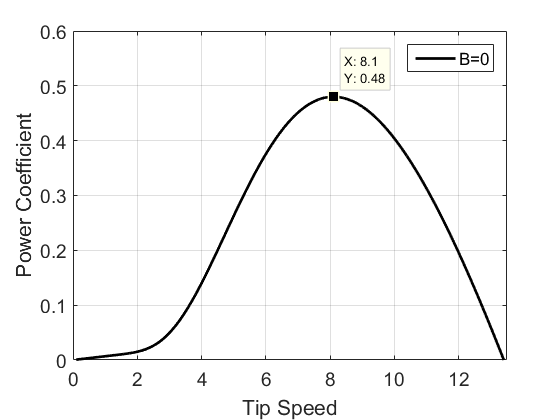
\includegraphics[width=.65\linewidth]{PowerCoefficient.png}
	\caption{Power Coefficient Variation with Tip Speed Ratio under Zero Pitch Angle}
	\label{variationofcp}
\end{figure} 
Variation of power coefficient $C_{p}$ is given in Figure \ref{variationofcp}. For the zero pitch angle, power coefficient has the maximum value of 0.48 for the tip speed ratio of 8.1. In order to ensure that the maximum of wind power is extracted, wind turbine should rotate a speed that gives the optimum tip speed ratio. 

\subsection{Gearbox}  
Variable speed PMSG wind turbines have a gearbox between turbine and generator except for direct-drive wind turbines. The gearbox increases angular speed and decreases the torque in the generator side.By decreasing the rated torque, generator size and cost can be reduced since the generator size is almost proportional to rated torque due to constant shear stress \cite{Polinder2013aa}.
\begin{figure}[h!]
	\centering
	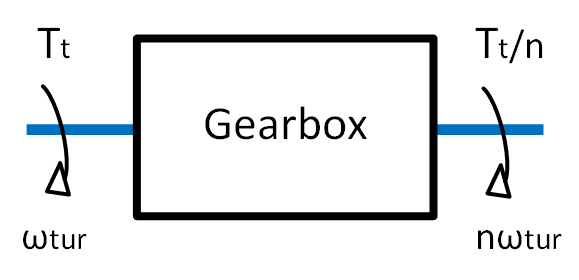
\includegraphics[width=.45\linewidth]{gearbox.png}
	\caption{Gearbox Modelling}
	\label{gearboxmodel}
\end{figure}

\subsection{Permanent Magnet Synchronous Generator}  